
Let us first look at the penalty formulation. In this case we are only solving for 
velocity since pressure is recovered in a post-processing step. We also know that 
the penalty factor is many orders of magnitude higher than the viscosity and 
in combination with the use of the $Q_1 \times P_0$ element the resulting matrix 
condition number is very high so that the use of iterative solvers in precluded. 
Indeed codes such as SOPALE \cite{full95}, DOUAR \cite{brtf08}, or FANTOM \cite{thie11} 
relying on the penalty formulation all use direct solvers (BLKFCT, MUMPS, WSMP).

The main advantage of direct solvers is used in this case: They can solve ill-conditioned 
matrices. However memory requirements for the storage of number of nonzeros in the 
Cholesky matrix grow very fast as the number of equations/grid size increases, especially in 3D,
to the point that even modern computers with tens of Gb of RAM cannot deal with a $100^3$ element mesh.
This explains why direct solvers are often used for 2D problems and rarely in 3D with noticeable 
exceptions \cite{thfb08,yahb09,brya09,lobh10,alht11,alht12,alhf13,whbb14,neew18}. 

In light of all this, let us start again from the (full) Stokes system:
\[
\left(
\begin{array}{cc}
\K & \G \\ \G^T & 0 
\end{array}
\right)
\cdot
\left(
\begin{array}{c}
{\cal V} \\ {\cal P}
\end{array}
\right)
=
\left(
\begin{array}{c}
 f \\ h
\end{array}
\right)
\]
We need to solve this system in order to obtain the solution, i.e. the ${\cal V}$ 
and ${\cal P}$ vectors. But how? 

Unfortunately, this question is not simple to answer and the 'right' depends on many 
parameters. 
How big is the matrix ? what is the condition number of the matrix $\K$ ? 
Is it symmetric ? (i.e. how are compressible terms handled?). 


%--------------------------------------------
\subsubsection{The Schur complement approach}
Let us write the above system as two equations:
\begin{eqnarray}
\K {\cal V} + \G {\cal P} &=& f \\
\G^T {\cal V} \quad\quad &=& h 
\end{eqnarray}
The first line can be re-written ${\cal V}=\K^{-1} (f - \G {\cal P})$ and can be inserted in the second:
\[
\G^T {\cal V} =\G^T [ \K^{-1} (f - \G {\cal P}) ] = h 
\]
or, 

\begin{mdframed}[backgroundcolor=blue!5]
\[
\G^T K^{-1} \G {\cal P} = \G^T \K^{-1} f - h 
\]
\end{mdframed}
The matrix $\SSS= \G^T \K^{-1} \G $ is called the Schur complement. \index{Schur complement} 
It is Symmetric (since $\K$ is symmetric) and  Postive-Definite\footnote{$M$ 
positive definite $\iff$ $x^TMx>0$ $\forall \; x\in \mathbb{R}^n \setminus {\bm 0}$ }
(SPD) \index{SPD} if $Ker({\G})=0$. 
{\color{red} look in donea-huerta book for details}
Having solved this equation (we have obtained ${\cal P}$), the velocity can be recovered by solving 
$\K {\cal V} =f- \G {\cal P}$. 
For now, let us assume that we have built the $\SSS$ matrix and the right hand side $\tilde{f}=\G^T \K^{-1} f - h$.
We must solve $\SSS {\cal P} = \tilde{f}$.

\index{CG} \index{conjugate gradient}
Since $\SSS$ is SPD, the Conjugate Gradient (CG) method is very appropriate to solve this system. 
Indeed, looking at the definition of Wikipedia: {\it In mathematics, the conjugate gradient method is an algorithm for the numerical solution of particular systems of linear equations, namely those whose matrix is symmetric and positive-definite. The conjugate gradient method is often implemented as an iterative algorithm, applicable to sparse systems that are too large to be handled by a direct implementation or other direct methods such as the Cholesky decomposition. Large sparse systems often arise when numerically solving partial differential equations or optimization problems.}

The Conjugate Gradient algorithm is as follows:

\begin{center}
\frame{
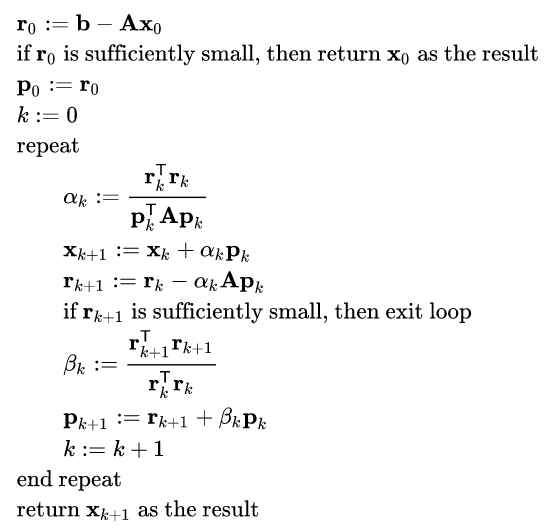
\includegraphics[width=6cm]{images/solvers/cgwiki}
}\\
Algorithm obtained from \url{https://en.wikipedia.org/wiki/Conjugate\_gradient\_method}
\end{center}

Let us look at this algorithm up close. The parts which may prove to be somewhat tricky 
are those involving the matrix (in our case the Schur complement).
We start the iterations with a guess pressure ${\cal P}_0$ (
and an initial guess velocity which could be obtained by solving $\K {\cal V}_0 =f- \G {\cal P}_0$).
\begin{eqnarray}
r_0 
&=& \tilde{f}-\SSS {\cal P}_0 \\
&=& \G^T \K^{-1} f - h - (\G^T \K^{-1} \G ) {\cal P}_0 \\ 
&=& \G^T \K^{-1} (f - \G {\cal P}_0) - h \\
&=& \G^T \K^{-1} \K {\cal V}_0 - h \\ 
&=& \G^T {\cal V}_0 - h \\ 
\end{eqnarray}
We now turn to the $\alpha_k$ coefficient:
\[
\alpha_k 
= \frac{r_k^T r_k }{p_k \SSS p_k } 
= \frac{r_k^T r_k }{p_k \G^T \K^{-1} \G  p_k } 
= \frac{r_k^T r_k }{(\G p_k)^T  \K^{-1} (\G  p_k) } 
\]
We then define $\tilde{p}_k = \G p_k$, so that $\alpha_k$ can be computed as follows:
\begin{enumerate}
\item compute $\tilde{p}_k = \G p_k$
\item solve $\K d_k = \tilde{p}_k$
\item compute $\alpha_k=(r_k^T r_k)/(\tilde{p}_k^T d_k)$
\end{enumerate}
Then we need to look at the term $\SSS p_k$:
\[
\SSS p_k = \G^T \K^{-1} \G p_k = \G^T \K^{-1} \tilde{p}_k = \G^T d_k
\]
We can then rewrite the CG algorithm as follows:
\begin{itemize}
\item $r_0 = \G^T {\cal V}_0 - h$ 
\item if $r_0$ is sufficiently small, then return $({\cal V}_0,{\cal P}_0)$ as the result
\item $p_0=r_0$
\item $k=0$
\item repeat
\begin{itemize}
\item compute $\tilde{p}_k = \G p_k$
\item solve $\K d_k = \tilde{p}_k$
\item compute $\alpha_k=(r_k^T r_k)/(\tilde{p}_k^T d_k)$
\item ${\cal P}_{k+1} = {\cal P}_k+\alpha_k p_k$
\item $r_{k+1} = r_k - \alpha_k \G^T d_k $
\item if $r_{k+1}$ is sufficiently small, then exit loop
\item $\beta_k=(r_{k+1}^T r_{k+1})/(r_k^T r_k)$
\item $p_{k+1} =r_{k+1}+ \beta_k p_k$
\item $k=k+1$
\end{itemize}
\item return ${\cal P}_{k+1}$ as result
\end{itemize}
We see that we have managed to solve the Schur complement equation with the Conjugate Gradient method
without ever building the matrix $\SSS$. Having obtained the pressure solution, we can easily recover the corresponding velocity with $\K {\cal V}_{k+1} =f- \G {\cal P}_{k+1}$. However, this is rather unfortunate because it requires yet another solve with the $\K$ matrix. As it turns out, we can slightly alter the above algorithm to have it update the velocity as well so that this last solve is unnecessary.

We have 
\[
{\cal V}_{k+1} 
= \K^{-1} (f - \G {\cal P}_{p+1} )
= \K^{-1} (f - \G ({\cal P}_k+\alpha_k p_k) )
= \K^{-1} (f - \G {\cal P}_k) - \alpha_k \K^{-1} \G p_k 
= {\cal V} - \alpha_k \K^{-1} \tilde{p}_k 
= {\cal V}_k - \alpha_k d_k 
\] 
and we can insert this minor extra calculation inside the algorithm and get the velocity solution 
nearly for free. The final CG algorithm is then 

\begin{mdframed}[backgroundcolor=blue!5]
\underline{\bf solver\_cg}:
\begin{itemize}
\item compute ${\cal V}_0=\K^{-1}(f-\G{\cal P}_0)$
\item $r_0 = \G^T {\cal V}_0 - h$ 
\item if $r_0$ is sufficiently small, then return $({\cal V}_0,{\cal P}_0)$ as the result
\item $p_0=r_0$
\item $k=0$
\item repeat
\begin{itemize}
\item compute $\tilde{p}_k = \G p_k$
\item solve $\K d_k = \tilde{p}_k$
\item compute $\alpha_k=(r_k^T r_k)/(\tilde{p}_k^T d_k)$
\item ${\cal P}_{k+1} = {\cal P}_k+\alpha_k p_k$
\item $ {\cal V}_{k+1} = {\cal V}_k - \alpha_k d_k$
\item $r_{k+1} = r_k - \alpha_k \G^T d_k $
\item if $r_{k+1}$ is sufficiently small ($|r_{k+1}|_2/|r_0|_2 <tol$), then exit loop
\item $\beta_k=(r_{k+1}^T r_{k+1})/(r_k^T r_k)$
\item $p_{k+1} =r_{k+1}+ \beta_k p_k$
\item $k=k+1$
\end{itemize}
\item return ${\cal P}_{k+1}$ as result
\end{itemize}
\end{mdframed}

This iterative algorithm will converge to the solution with a rate which depends on 
the condition number of the $\SSS$ matrix, which is not easily obtainable since 
$\SSS$ is never built. Also, we know that large viscosity contrasts in the domain 
will influence this too. Finally, we notice that this algorithm requires one solve
with matrix $\K$ per iteration but says nothing about the method employed to do so.

One thing we know improves the convergence of any iterative solver is the use of a 
preconditioner matrix.  





\improvement[inline]{repeat for PCG}









\subsection{The GMRES approach}
